\chapter{要素技術}
\label{technical_background}

本章では本研究に用いる手法に関連する要素技術について述べる


\section{機械学習}

機械学習とは広義には, コンピューターが自動的にパターンを学習し人間による明示的な命令がなくとも
特定の課題を自動で実行する技術又はアルゴリズムのことである. 主に, 正解データを与えることによってパターンを学習する教師あり学習,
データのまとまりや相関を求める教師なし学習と繰り返し反復することで価値が最大化するように学習を行う強化学習に分類される.
画像処理や自然言語処理など様々な分野に応用が進んでおり, 画像の検知や自動翻訳など機械学習によって自動化されているものも多い.


\subsection{深層学習}

深層学習とは脳が持つ脳神経系のニューロンをソフトウェアで再現した人工ニューラルネット(ANN)を持つ機械学習アルゴリズムの一つである. 
人間の脳を模したパーセプトロン~\cite{Perceptron}による深層学習自体は1957年から提唱されていた. しかし, 4層以上のパーセプトロンでは過学習や勾配消失問題が発生しやすく計算コストも大きいためあまり普及しなかった.
しかし, 安価なコンピューターでも計算速度が飛躍的に向上したことや勾配消失問題を防止する手法が考案されたことなどから再び注目を集めるようになり, 様々な課題に特価したDNNが考案されている.

例えば, Convolutional Neural Network (CNN)~\cite{CNN}は画像の特徴量抽出に長けており画像認識分野で大きな成果をあげている.
Long short-term memory (LSTM) ~\cite{LSTM}は自動翻訳やテキスト解析など自然言語処理分野で活用されており, 現在では言語だけではなく音楽などにも活用範囲が広がっている.
また, 既存の機械学習の手法に深層学習を組み込んだ事例も散見される.

\subsection{多層パーセプトロン}
パーセプトロンとは


\begin{figure}[H]
    \centering
    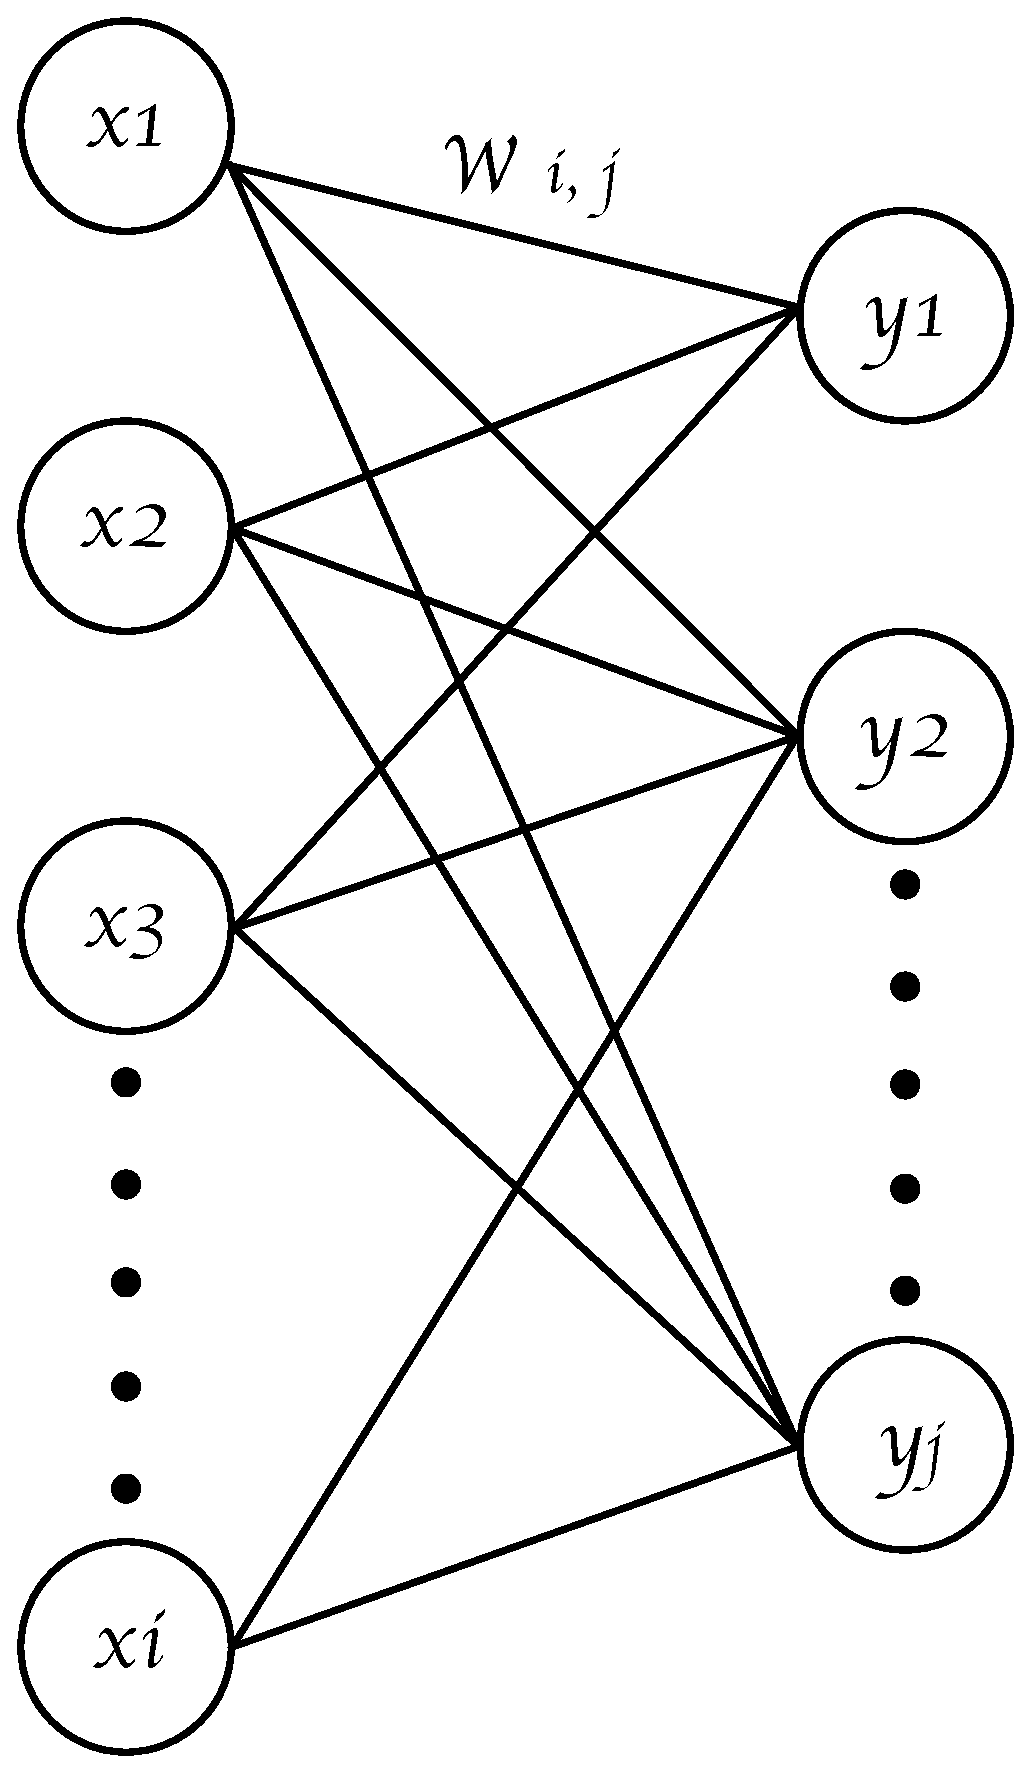
\includegraphics[clip,height = 8.0cm]{assets/perceptron.eps}
    \caption{パーセプトロン}  \label{sample}
\end{figure}

\subsection{強化学習}

強化学習 (Reinforcement learning) ~\cite{ReinforcementLearning}はエージェントと呼ばれる行動主体が現在の状態を観測し価値が最大化する行動を繰り返し選択することにより利益が最大になる行動を学習する機械学習手法の一種である.
強化学習では行動主体であるエージェントと環境を定義する状態と行動した結果による変化, 報酬が定義される.
初期的な強化学習にはマルコフ決定過程~\cite{ReinforcementLearning}やQ学習~\cite{QL}というものがある.

\subsection{深層強化学習}

深層強化学習とは, 強化学習に深層学習を組み合わせた機械学習アルゴリズムである.
強化学習はエージェントとエージェントが動作する環境を定義し, 定義された環境下でエージェントへの報酬が最大化するように学習は行う.

\begin{figure}[H]
    \centering
    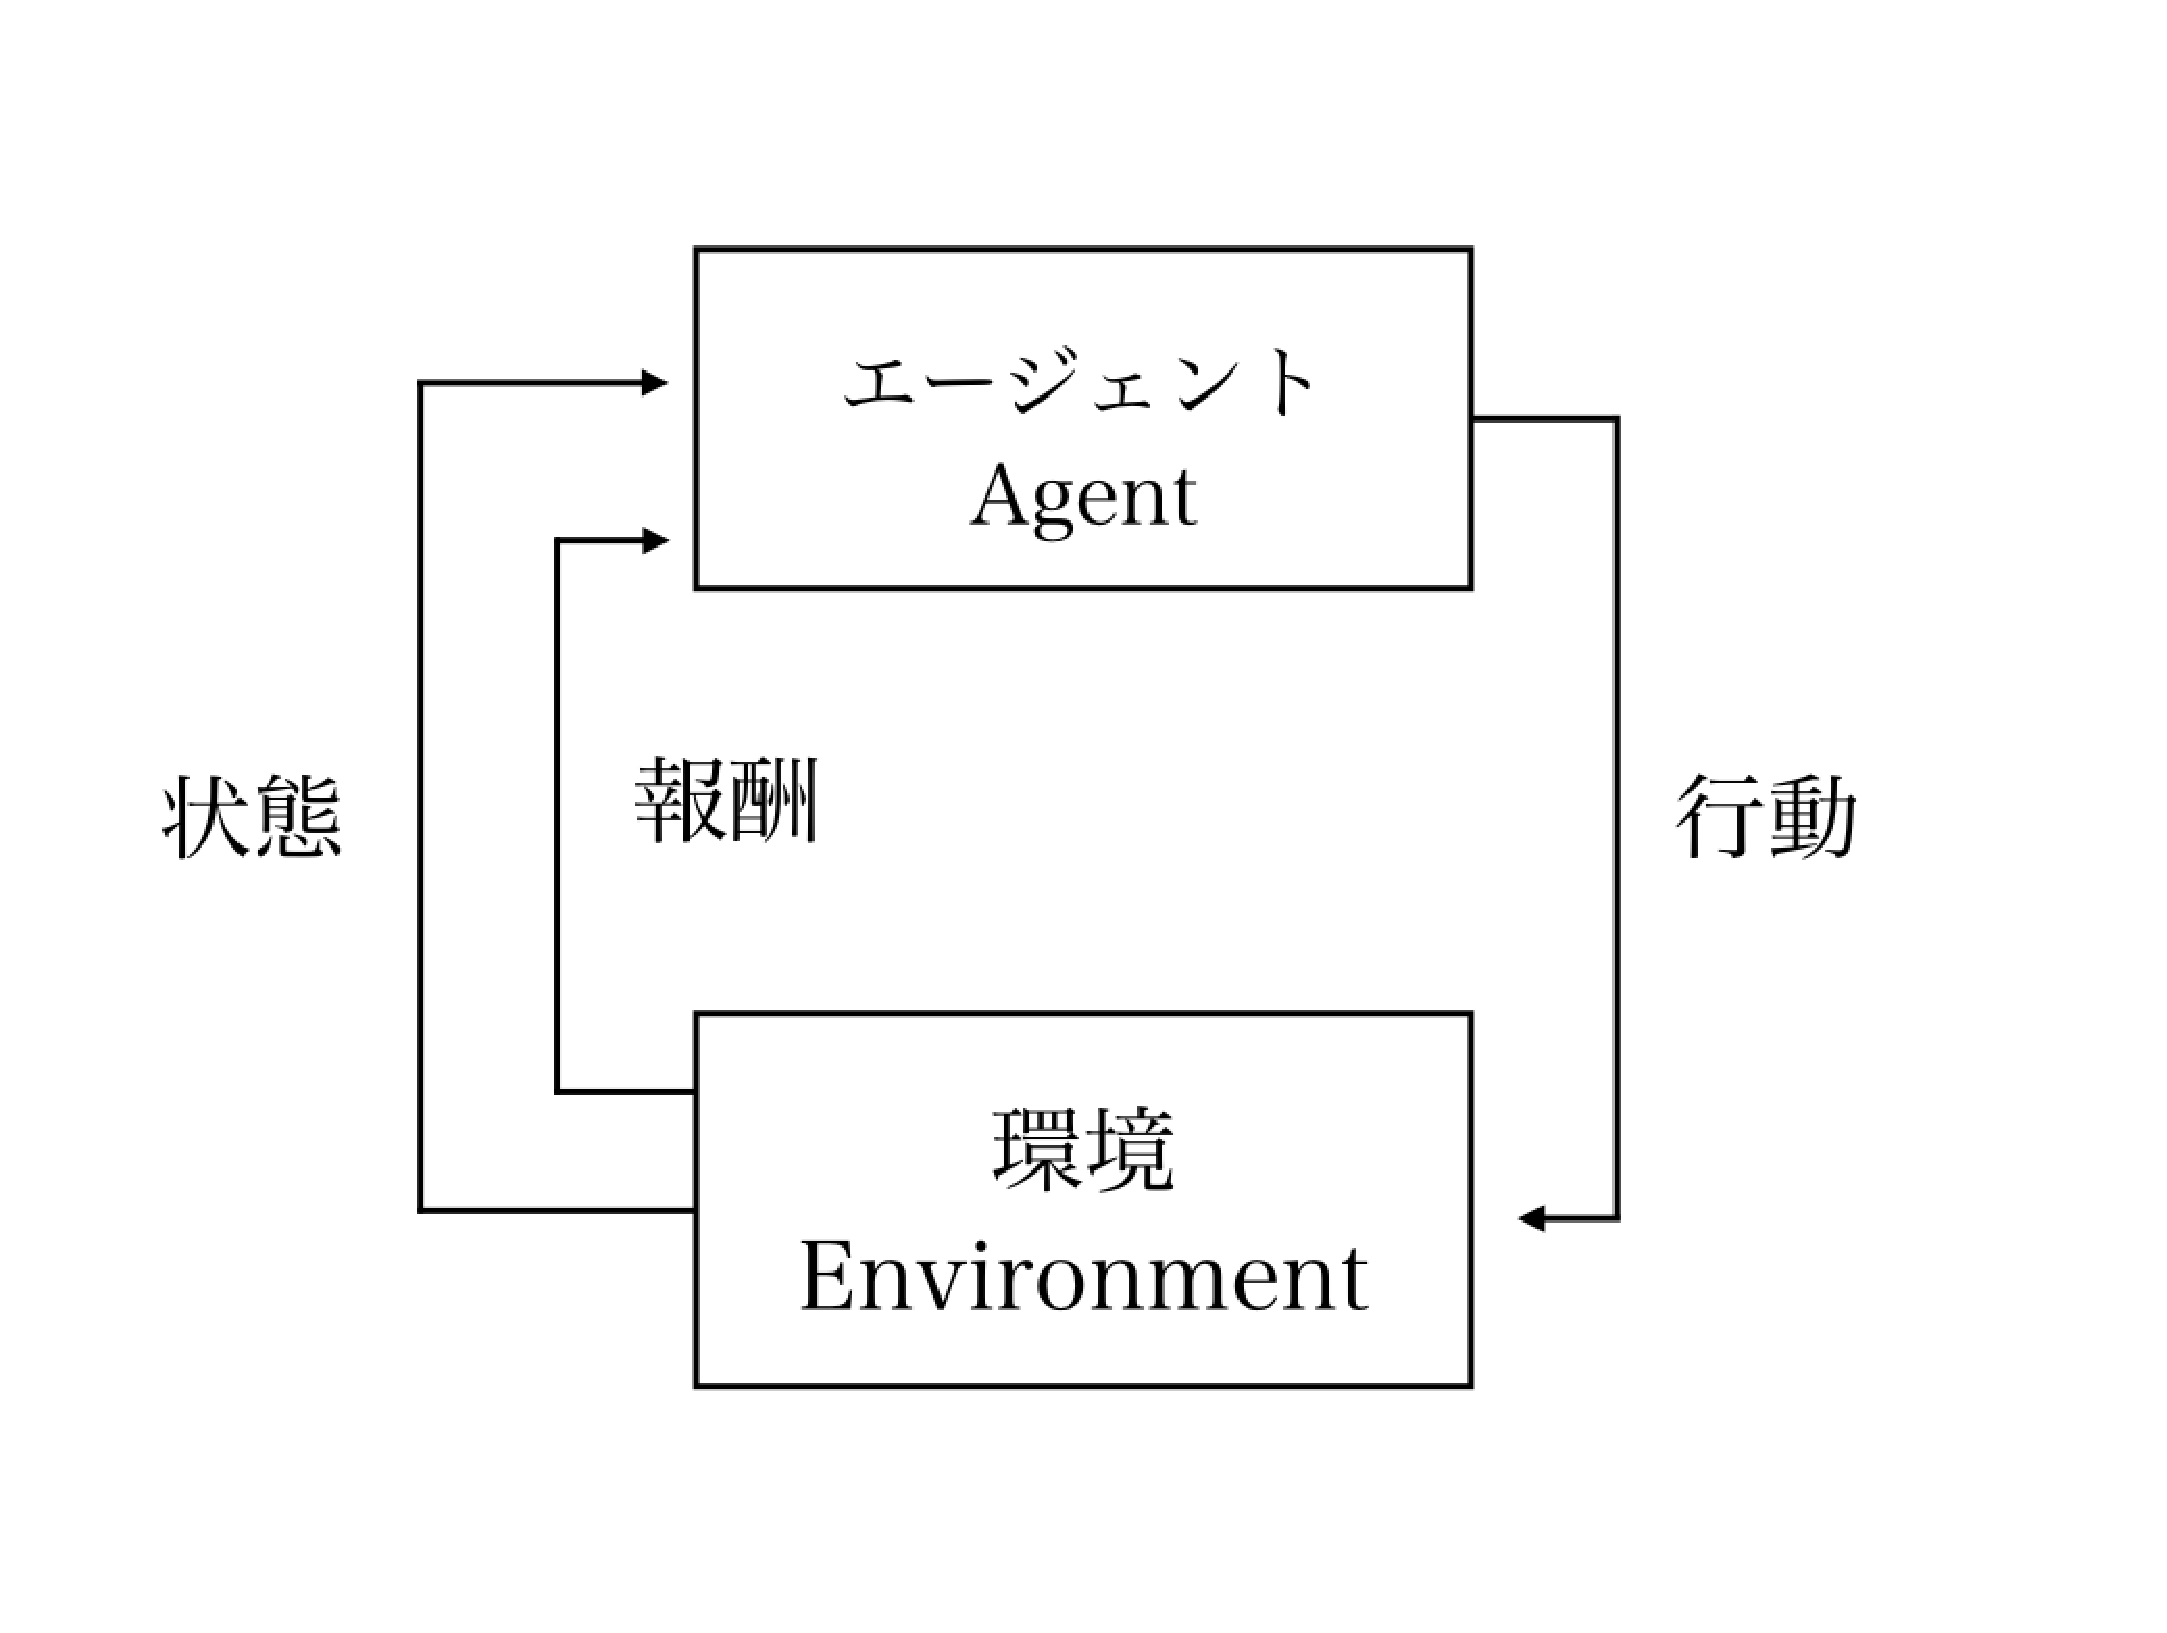
\includegraphics[clip,width = 12.0cm]{assets/reinforcement_learning.eps}
    \caption{強化学習の概念図}  \label{sample}
\end{figure}

\section{Q学習}

Q学習とは初期に考案されたReinforest Learningアルゴリズムの一種であり, 強化学習と呼ばれす.
Q学習による試行は以下のように定義する.

\begin{equation}
    Q(s, a) \approx R(s, a) + \gamma max_{a'} E[Q(s', a')]
\end{equation}

\section{Deep Q Neural Network}

Deep Q Neural Network(DQN~\cite{DQN})の一種でQ学習という強化学習における古典的なアルゴリズムを深層強化学習に応用したものである.
\textcolor{red}{ちょと再考}
Q学習~\cite{QL}とは強化学習の一種である. Q学習~\cite{QL}では実行するルールに対してQ値という値を持たせる.

DQNの深層学習部分はCNN~\cite{DQN}で構成される.

\begin{figure}[H]
    \centering
    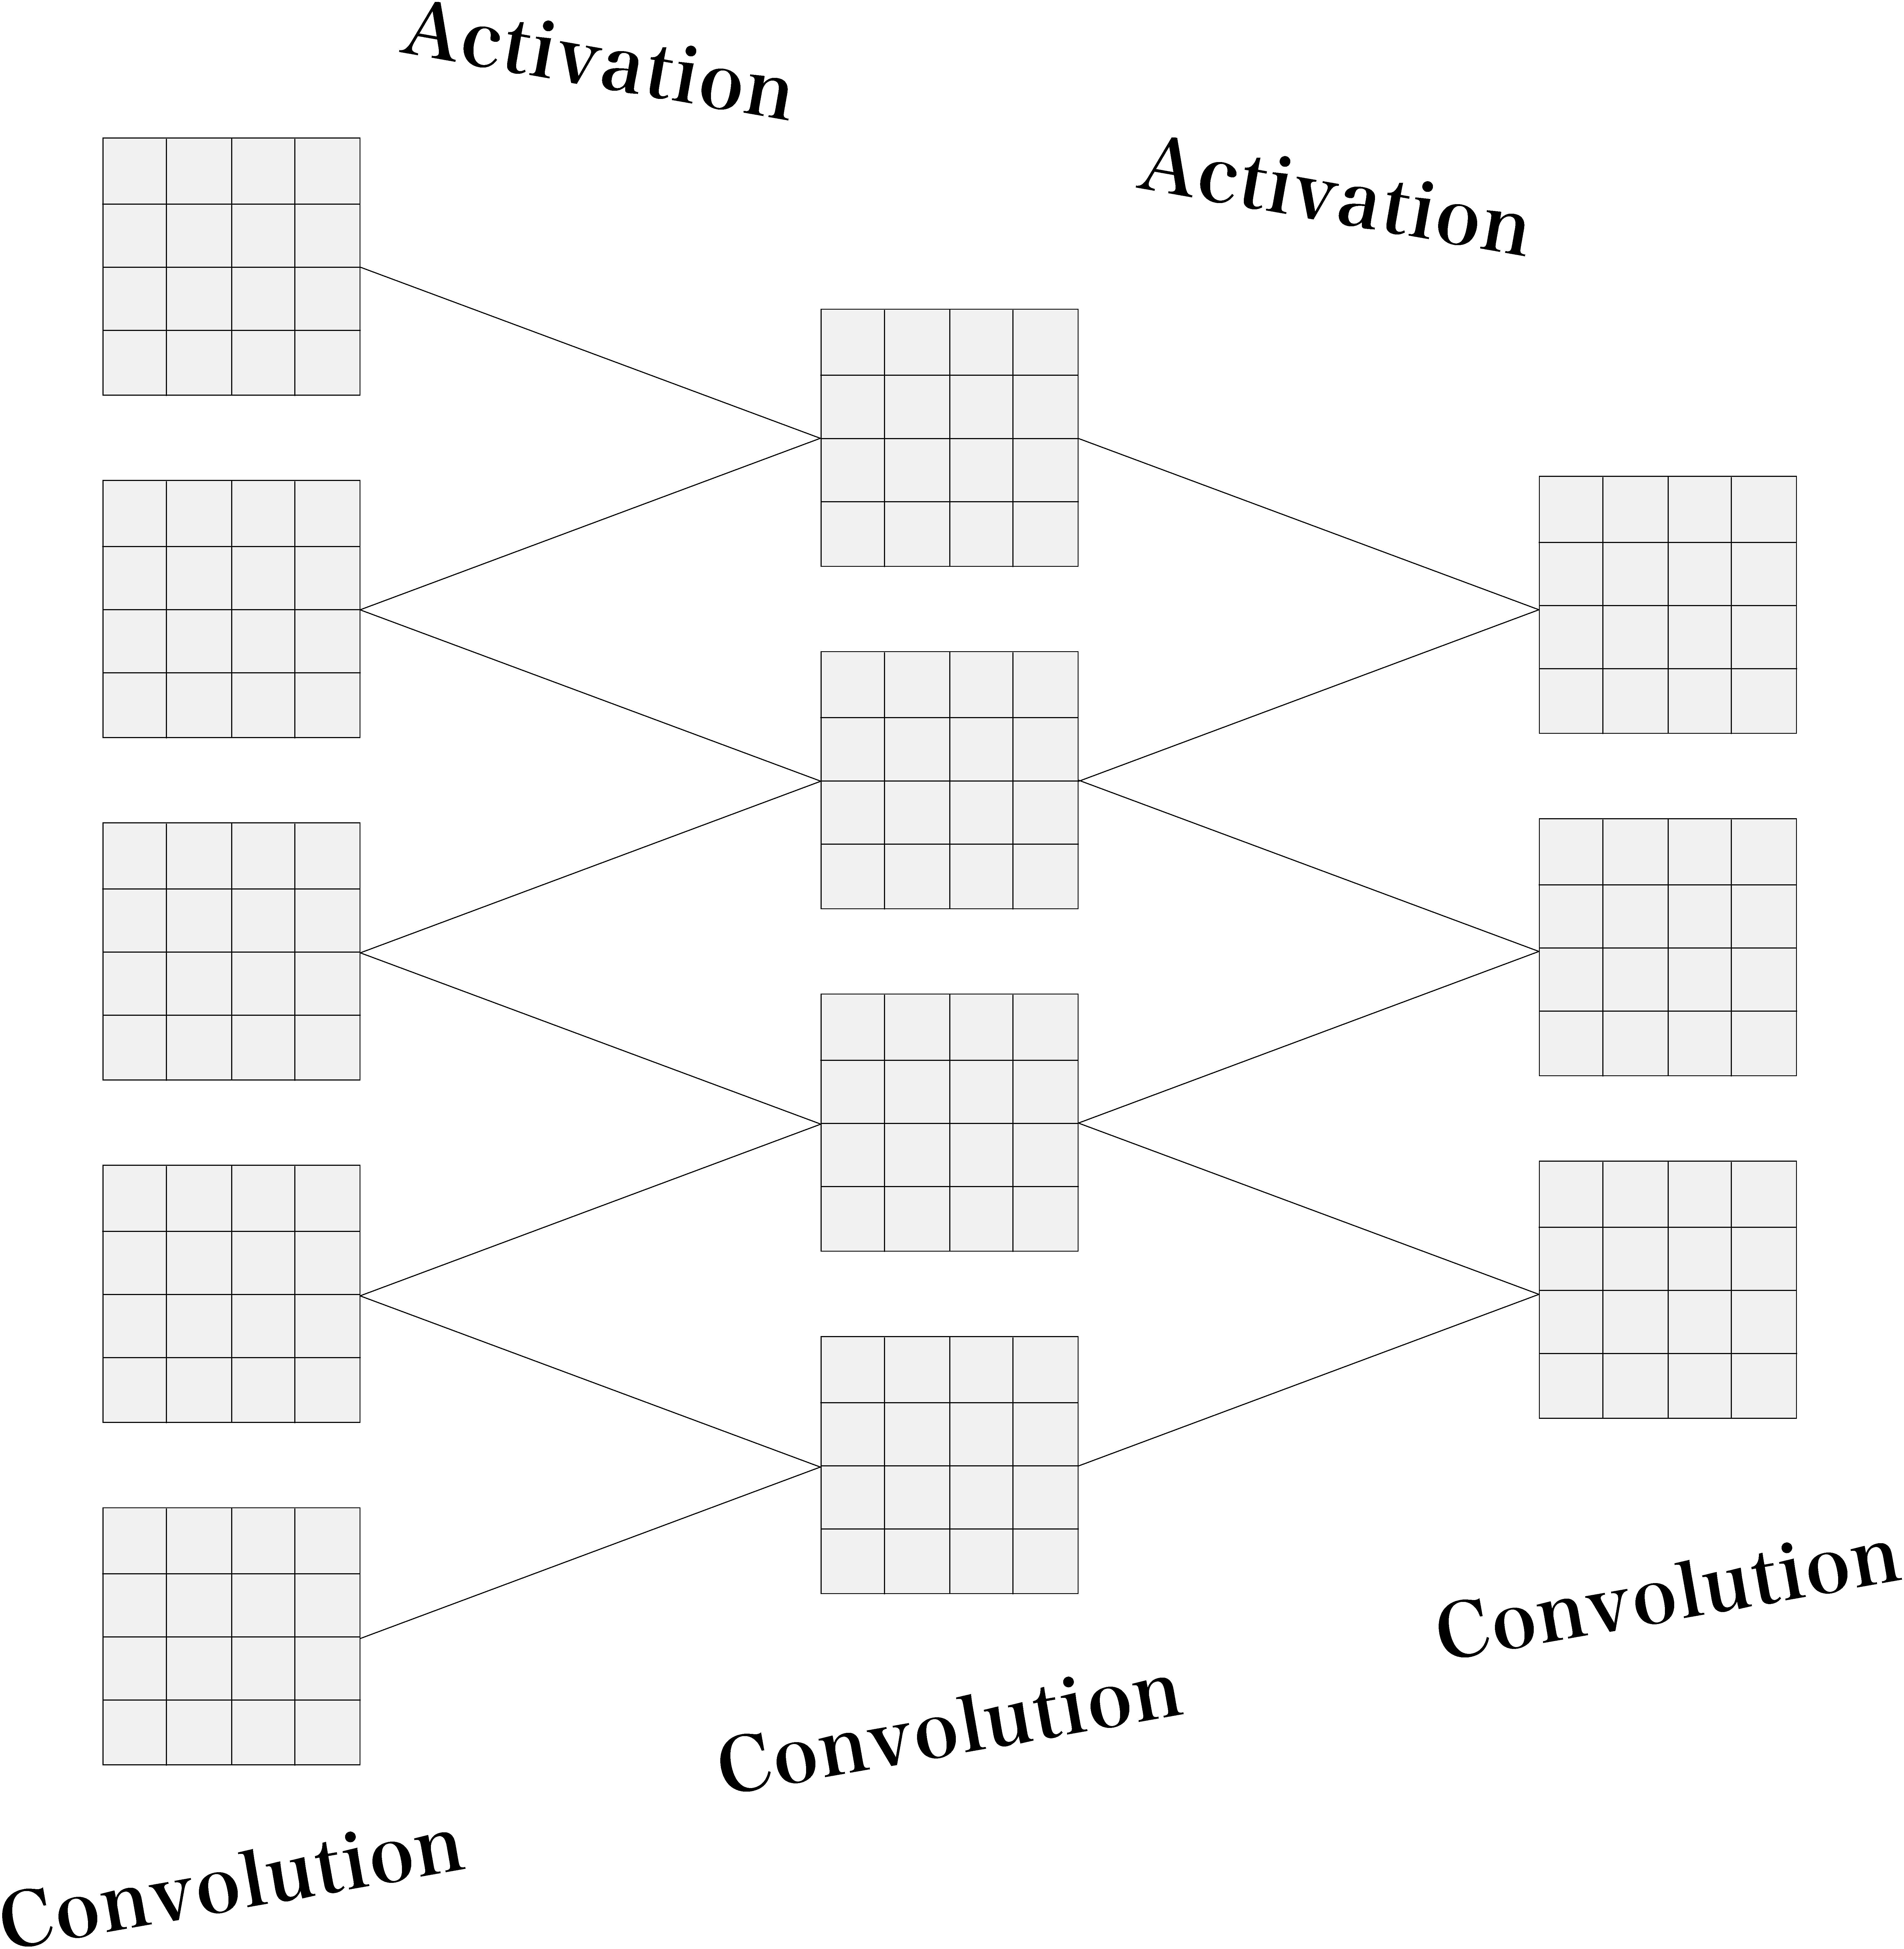
\includegraphics[clip,height = 8.0cm]{assets/dqn_convolution.eps}
    \caption{DQNを構成するCNN}  \label{sample}
\end{figure}




\begin{figure}[H]
    \centering
    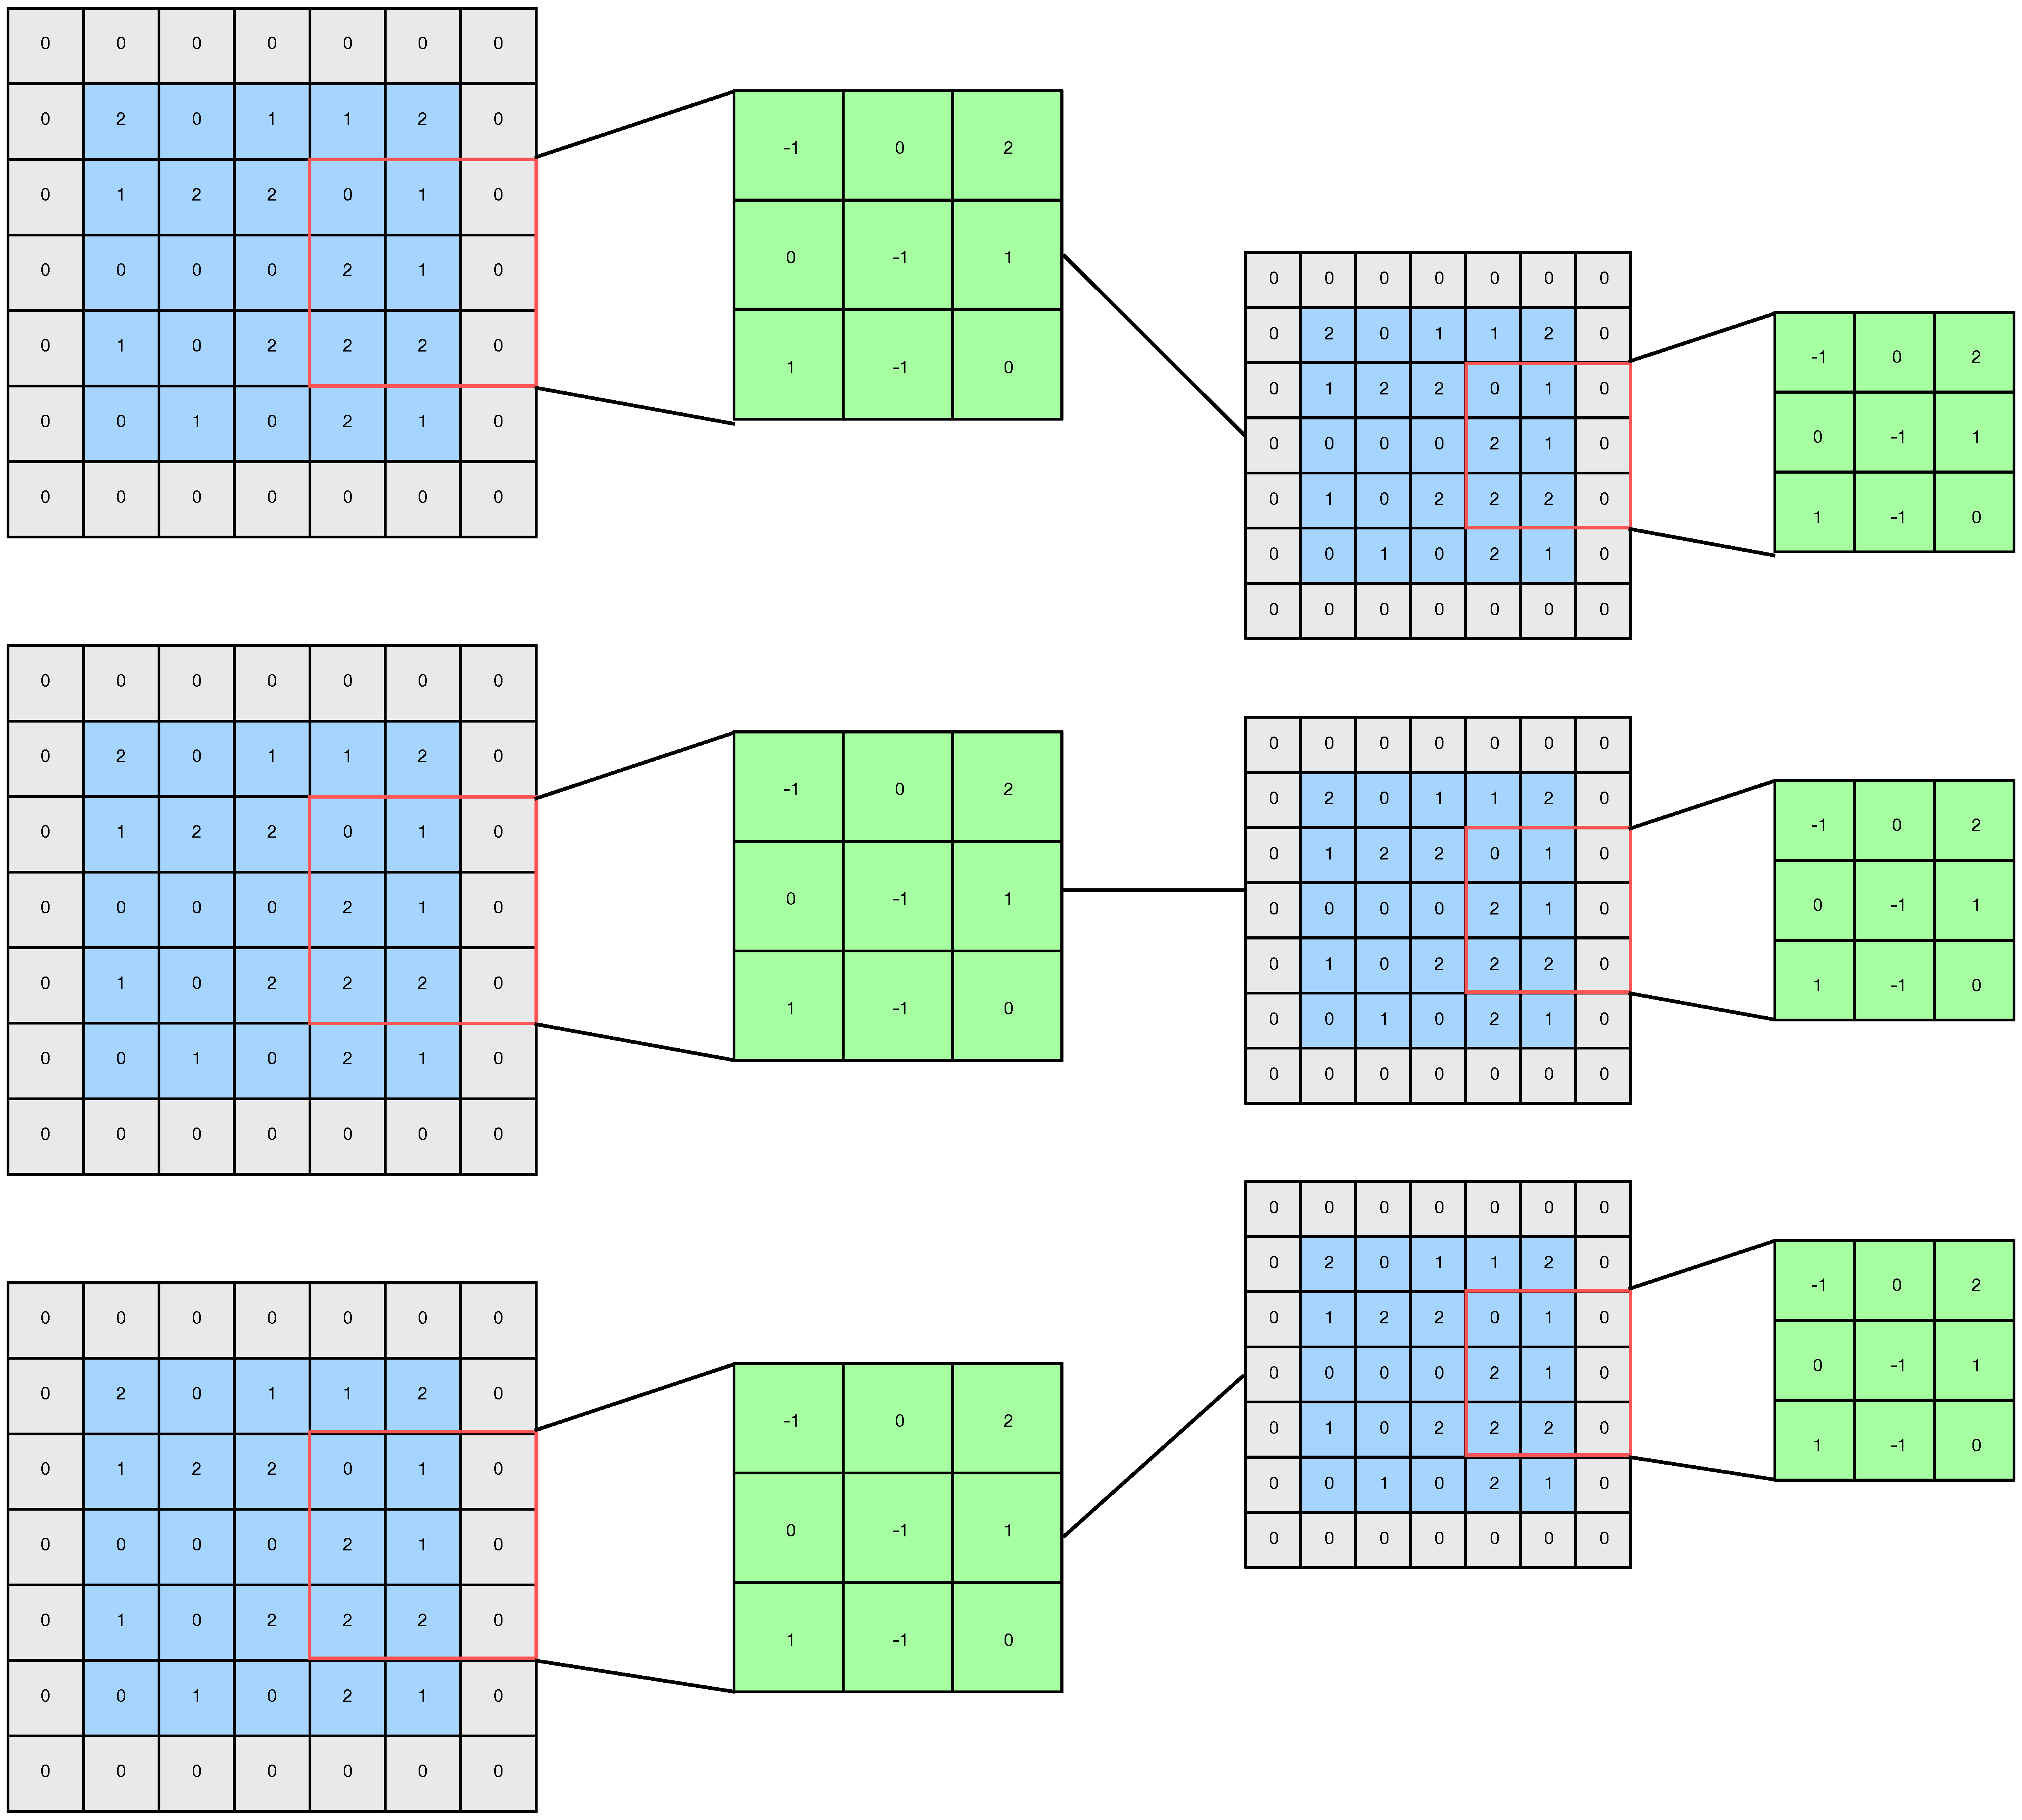
\includegraphics[clip,height = 8.0cm]{assets/CNN_typical.eps}
    \caption{一般的なConvolutional Neural Network}  \label{sample}
\end{figure}



%%% Local Variables:
%%% mode: japanese-latex
%%% TeX-master: "../bthesis"
%%% End:
